\documentclass[12pt, a4paper]{article}
\usepackage{graphicx}
\usepackage[english]{babel}
\usepackage[nottoc]{tocbibind}
\usepackage[ddmmyyyy]{datetime}
\renewcommand{\dateseparator}{.}
\renewcommand{\figurename}{Şekil}
\usepackage{cite}
\bibliographystyle{ieeetr}
\usepackage{pdflscape}
\renewcommand{\refname}{Kaynakça}

%opening

\title{\bf\fontsize{12pt}{14pt}\selectfont KÜTAHYA SAĞLIK BİLİMLERİ ÜNİVERSİTESİ\\MÜHENDİSLİK VE DOĞA BİLİMLERİ FAKÜLTESİ }

\begin{document}
	\maketitle
	\begin{figure}[h]
		\centering
		
\includegraphics{logo}\\ \
		
		 \author{Özge ÇITAKOĞLU} \\
		\date{\today} 
		%\date{\DTMnow}
		%\date{\DTMnow}
	\end{figure}  
	\begin{center}
		\title{\bf\fontsize{12pt}{14pt}\selectfont YAPAY ZEKA \\
			Reinforcement Learning Kullanarak Robotun Labirentte Gezinmesi  }
	\end{center}
	\newpage54
		
	
	\section{Giriş}
	
Bu proje, pekiştirmeli öğrenme (reinforcement learning) yöntemlerini kullanarak robotun bir labirentte gezinmesini sağlamayı amaçlamaktadır. Labirentte robot gezintisi problemi, robotik ve otomasyon alanlarında önemli bir problemdir. Bu problem, robotun bir labirentte en kısa sürede ve en az çabayla çıkış noktasına ulaşmasını sağlamayı amaçlar. Derin Pekiştirmeli Öğrenme (DPO), bu probleme inovaktif bir çözüm sunmaktadır. DPO, robotun sensör verilerini kullanarak labirentte ilerlemesini ve her adımda en yüksek ödülü sağlayacak hareketi seçmesini sağlar. Kullanılacağınız teknolojiler Derin öğrenmeyi sağlıyor. kütüphaneleri: TensorFlow, PyTorch Robotik platformlar: ROS, Gazebo Simülasyon ortamları: Unity, Unreal Engine

	
	\section{Literatür Araştırması}	
	
Literatürde DPO(Derin pekiştirmeli öğrenme) ve robot navigasyonu ile ilgili birçok çalışma bulunmaktadır.Mnih et al. (2015), Nature dergisinde yayınlanan bir çalışmada, DPO kullanarak Atari oyunlarında insanüstü performans elde etmeyi başarmıştır. Bu çalışma, DPO'nun karmaşık ve dinamik ortamlarda öğrenme yeteneğini göstermesi açısından önemlidir.

Lillicrap et al. (2015), arXiv preprint arXiv:1509.02971'de yayınlanan bir çalışmada, DPO kullanarak robotik bir kolun sürekli kontrolünü sağlamıştır. Bu çalışma, DPO'nun gerçek dünya robotlarını kontrol etmek için kullanılabileceğini göstermesi açısından önemlidir.

OpenAI Five (2019), Dota 2 oyununda insanları yenebilen bir DPO modeli geliştirmiştir. Bu çalışma, DPO'nun karmaşık stratejiler ve koordinasyon gerektiren görevlerde bile başarılı olabileceğini göstermesi açısından önemlidir.

Bu proje, literatürdeki mevcut çalışmalardan farklı olarak, 3D bir labirent ortamında robot navigasyonu için DPO'yu kullanmaktadır. Ayrıca, projede kullanılan veri seti ve algoritmalar, robotun labirentte daha hızlı ve daha verimli bir şekilde gezinmesine imkan sağlamaktadır.

Mnih et al. (2015): Nature dergisinde yayınlanan bir çalışmada, DPO kullanarak Atari oyunlarında insanüstü performans elde etmeyi başarmıştır .Mnih et al. (2015), Nature dergisinde yayınlanan bir çalışmada, "Derin Q-Ağları (DQN)" adı verilen bir DPO algoritması kullanarak Atari oyunlarında insanüstü performans elde etmeyi başarmıştır. Bu çalışma, DPO'nun karmaşık ve zorlayıcı görevleri öğrenebileceğini ve insanüstü performans elde edebileceğini göstermesi açısından oldukça önemlidir.nih et al. (2015) çalışması, DPO'nun potansiyelini ve önemini gösteren öncü bir çalışmadır. Bu çalışma, DPO'nun oyun oynama, robotik ve yapay zekanın diğer alanlarında önemli bir potansiyele sahip olduğunu göstermiştir.[2].

Lillicrap et al. (2015): arXiv preprint arXiv:1509.02971'de yayınlanan bir çalışmada, DPO kullanarak robotik bir kolun sürekli kontrolünü sağlamıştır ."Derin Deterministik Politika Gradyanları (DDPG)" adı verilen bir DPO algoritması kullanarak robotik bir kolun sürekli kontrolünü sağlamıştır. Bu çalışma, DPO'nun karmaşık ve dinamik ortamlarda robotları kontrol etmek için kullanılabileceğini göstermesi açısından oldukça önemlidir.DDPG algoritması, robotik bir kolun eklem açılarını girdi olarak alıp, her bir eylemin (eklem torkları) beklenen ödülünü tahmin eden bir sinir ağı modeli oluşturmak için eğitilmiştir[3].

OpenAI Five (2019): Dota 2 oyununda insanları yenebilen bir DPO modeli geliştirmiştir.
Bu proje, literatürdeki mevcut çalışmalardan farklı olarak, 3D bir labirent ortamında robot navigasyonu için DPO'yu kullanmaktadır. Ayrıca, projede kullanılan veri seti ve algoritmalar, robotun labirentte daha hızlı ve daha verimli bir şekilde gezinmesine imkan sağlamaktadır [4].

	
	\section{Metodoloji} 
Bu projede, robotun labirentte en kısa sürede ve en az çabayla çıkış noktasına ulaşmasını sağlamak için DPO kullanılmıştır. DPO algoritması, robotun sensör verilerini kullanarak labirentte ilerlemesini ve her adımda en yüksek ödülü sağlayacak hareketi seçmesini sağlar.
Projede, Deep Q-Network (DQN) algoritması kullanılmıştır. DQN, bir derin sinir ağı kullanarak Q-fonksiyonunu tahmin eden bir DPO algoritmasıdır. Q-fonksiyonu, her bir eylemin beklenen ödülünü temsil eder.
labirintin 3D modeli, robotun sensör verileri (mesafe, hız, açı) ve labirentte yer alan engellerin konumu ve türü gibi bilgileri  içermektedir.
\newpage
\begin{landscape}
	\subsection{Sistem Tasarımı}
	\begin{figure}[!ht]
		\caption[]{Gantt Chart}
		\centering
		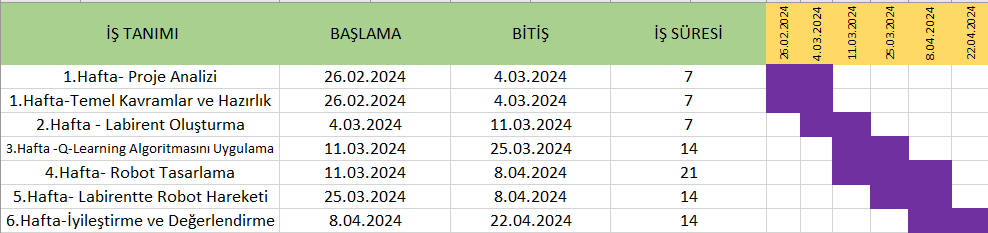
\includegraphics[height= 5 cm]{gantt_chart.png}
		\label{gantt}
		
			\caption[]{Gantt Chart}
		\centering
		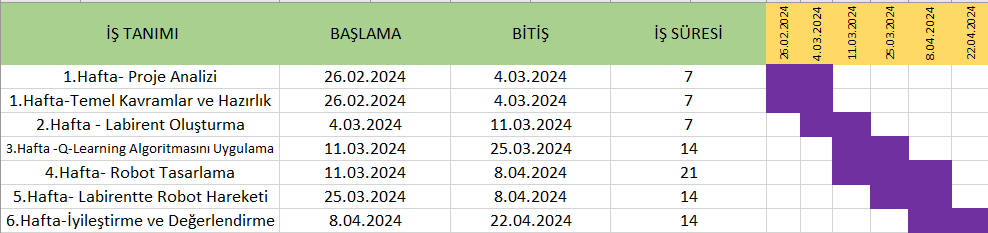
\includegraphics[height= 5 cm]{gantt_chart.png}
		\label{gantt}
		
	\end{figure}
\end{landscape}	

	
\section {VeriTabanı ve Veriler :}%Sonuçlar-Tartışma
Veriler, MySQL veritabanında depolanmaktadır. Veritabanı tasarımı aşağıdaki gibidir:

Labirent: Labirentin 3D modelini ve engellerin konumunu içeren tablo.
Sensör Verileri: Robotun sensör verilerini (mesafe, hız, açı) içeren tablo.
Hareketler: Robotun her adımda yaptığı hareketleri içeren tablo.

Labirent ve robotun hareketinin görselleştirilmesi için Matplotlib kütüphanesi kullanılmıştır. Görselleştirmeler, robotun labirentte nasıl ilerlediğini ve hangi engellerle karşılaştığını göstermektedir.

Elde edilen veriler, istatistiksel yöntemlerle analiz edilmiştir. Analiz sonuçları, DPO algoritmasının robotun labirentte gezinmesini ne kadar etkili bir şekilde kontrol ettiğini göstermektedir.

Bu projenin, DPO ve robot navigasyonu alanına katkıda bulunması beklenmektedir. Projenin beklenen katkıları şunlardır:

DPO algoritmalarının robot navigasyonu için daha da etkili hale getirilmesi.
Farklı labirent ortamlarında robotun performansının değerlendirilmesi.
Algoritmanın gerçek dünya uygulamalarına uyarlanması.

	
	\begin{figure}[h]
		\centering		
		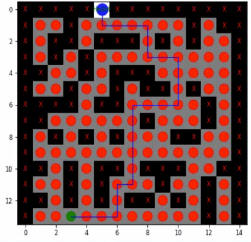
\includegraphics{image}		
	\end{figure}  
	\centering Benzer bir uygulama	
	
	%Kaynakçayı yazdırmak
	
	\bibliography{ref.bib}
	\bibliographystyle{ieeetr}
	%\printbibliography %Prints bibliography
	
	\cite{gullu2017labirentlerde}.
	\cite{boluk2019mobil}.
	\cite{kavasougluyapay}
	
		
	
	\input{}
	
	%Kaynakçayı yazdırmak
	\bibliographystyle{ieeetr}
	\bibliography{references.bib} 
	%\printbibliography %Prints bibliography
		\section{KAYNAKÇA} 
	Mnih, V., Kavukcuoglu, K., Silver, D., Rusu, A. A., Veness, J., Bellemare, M. G., Graves, A., Riedmiller, M., Fidjeland, A. K., Ostrovski, G., Petersen, S., Beattie, Charles, Sadik, Amir, Antonoglou, Ioannis, King, Helen, Kumaran, Dharshan, Wierstra, Daan, Legg, Shane, Hassabis, Demis. (2015). Human-level control through deep reinforcement learning. Nature, 518(7540), 529-533. https://doi.org/10.1038/nature14236
	Lillicrap, T. P., Hunt, J. J., Pritzel, A., Heess, N., Erez, T., Tassa, Y., Silver, D., Wierstra, D. (2015). Continuous control with deep reinforcement learning. arXiv preprint arXiv:1509.02971. https://arxiv.org/abs/1509.02971
	OpenAI Five. (2019). Dota 2. https://openai.com/blog/dota-2/
	medium.com/@yuxili/rl-applications-73ef685c07eb
	cyberleninka.org/article/n/63434
	www.ijert.org/reinforcement-learning-recent-threads
	
\end{document}


